\documentclass[10pt]{beamer}

\usetheme{metropolis}
\usepackage{appendixnumberbeamer}

\usepackage{booktabs}
\usepackage[scale=2]{ccicons}
\usepackage{graphicx}
\usepackage{hyperref}
\usepackage{circuitikz}
\usepackage{pdflscape}
\usepackage{smartdiagram}

\usepackage{color}
\usepackage{listings}

\lstset{
	basicstyle=\footnotesize\ttfamily,
    keepspaces=true,
    showstringspaces=false,
    language=PHP,
    commentstyle=\ttfamily,
}

\usepackage[OT4]{polski}
\usepackage[utf8]{inputenc}

\usepackage{pgfplots}
\usepgfplotslibrary{dateplot}

\usepackage{xspace}
\newcommand{\themename}{\textbf{\textsc{metropolis}}\xspace}

\setbeamertemplate{frame footer}{}
\setbeamertemplate{frame numbering}{}

\usetikzlibrary{shapes,arrows}

\tikzstyle{decision} = [diamond, draw, fill=blue!20, 
    text width=4.5em, text badly centered, node distance=3cm, inner sep=0pt]
\tikzstyle{block} = [rectangle, draw, fill=blue!20, 
    text width=5em, text centered, rounded corners, minimum height=4em]
\tikzstyle{line} = [draw, -latex']
\tikzstyle{cloud} = [draw, ellipse,fill=red!20, node distance=3cm,
    minimum height=2em]


\title{Środowiska deweloperskie, testowe i produkcyjne}

\subtitle{Projektowanie i programowanie systemów internetowych I}
\author{mgr inż. Krzysztof Rewak}
\date{\today}
\institute{Wydział Nauk Technicznych i Ekonomicznych \\ Państwowa Wyższa Szkoła Zawodowa im. Witelona w Legnicy}

\begin{document}

\maketitle

\begin{frame}{Plan prezentacji}
  \setbeamertemplate{section in toc}[sections numbered]
  \tableofcontents[hideallsubsections]
\end{frame}


\section{Środowisko programistyczne}

\begin{frame}[fragile]{Budowa klasycznego systemu internetowego}
	\begin{tikzpicture}[node distance=3cm, minimum size=2cm, auto]
	
		\node [block] (core) {jądro systemu};
	
		\node [block, above of=core] (server) {funkcje serwerowe};
		\node [block, left of=core] (database) {bazy danych};
		\node [block,above left of=core] (cache) {serwery cache};
		\node [block, below left of=core] (filesystem) {systemy plików};
		\node [block, below of=core] (services) {inne serwisy};
	
		\path [line] (core) -- node {} (server);
		\path [line] (server) -- node {} (core);
	
		\path [line] (core) -- node {} (database);
		\path [line] (database) -- node {} (core);
	
		\path [line] (core) -- node {} (cache);
		\path [line] (cache) -- node {} (core);
	
		\path [line] (core) -- node {} (filesystem);
		\path [line] (filesystem) -- node {} (core);
	
		\path [line] (core) -- node {} (services);
		\path [line] (services) -- node {} (core);
		
		\node [circle, fill=orange,inner sep=3pt, right of=core] (http) {serwer HTTP};
	
		\path [line] (http) -- node {} (core);
		\path [line] (core) -- node {} (http);
		
		\node [block, above right of=http] (browser) {przeglądarka};
		\node [block, below right of=http] (api) {inna aplikacja};
	
		\path [line] (http) -- node {} (browser);
		\path [line] (browser) -- node {} (http);
	
		\path [line] (http) -- node {} (api);
		\path [line] (api) -- node {} (http);
	
	\end{tikzpicture}
\end{frame}

\begin{frame}{\emph{Dramatis personae}}
	Na co między innymi powinniśmy zwrócić uwagę?
	\begin{itemize}
		\item rodzaj, wersja i konfiguracja serwera
		\item wersja języka lub interpretera
		\item zainstalowane programy
		\item wersja i typ bazy danych
		\item wersja frameworka
		\item zakres funkcjonalności
	\end{itemize}
\end{frame}

\begin{frame}{(uogólniona) Definicja}
	Środowiskiem programistycznym możemy uogólniając nazwać zestaw konkretnych programów, ich wersji oraz ich konfiguracji.
\end{frame}

\begin{frame}{Pierwsze problemy}
	Pierwszy problem pojawi się w momencie zaistnienia różnic między środowiskiem jakie mamy na komputerze przy którym pracujemy a środowiskiem na maszynie, na której system będzie działał docelowo.
\end{frame}

\begin{frame}{Więcej problemów?}
	\emph{U mnie działa} już dawno temu przestało być wiarygodną wymówką.
	
	Profesjonalista powinien przedstawić klientowi swoją aplikację. Ale jak to sensownie zrobić, jeżeli klient mieszka hen daleko w Honolulu, więc nie możemy odwiedzić go z naszym laptopem?
\end{frame}

\begin{frame}{Rozwiązanie jest proste}
	Aby usprawić proces wytwarzania oprogramowania, przyjęto schemat pracy z wieloma środowiskami programistycznymi, które są ze sobą powiązane w konkretny sposób. Należy wyróżnić środowiska:
	\begin{itemize}
		\item lokalne
		\item deweloperskie
		\item testowe
		\item \emph{stagingowe}
		\item produkcyjne
	\end{itemize}
\end{frame}

\begin{frame}[fragile]{Co, gdzie, kiedy, jak?}
	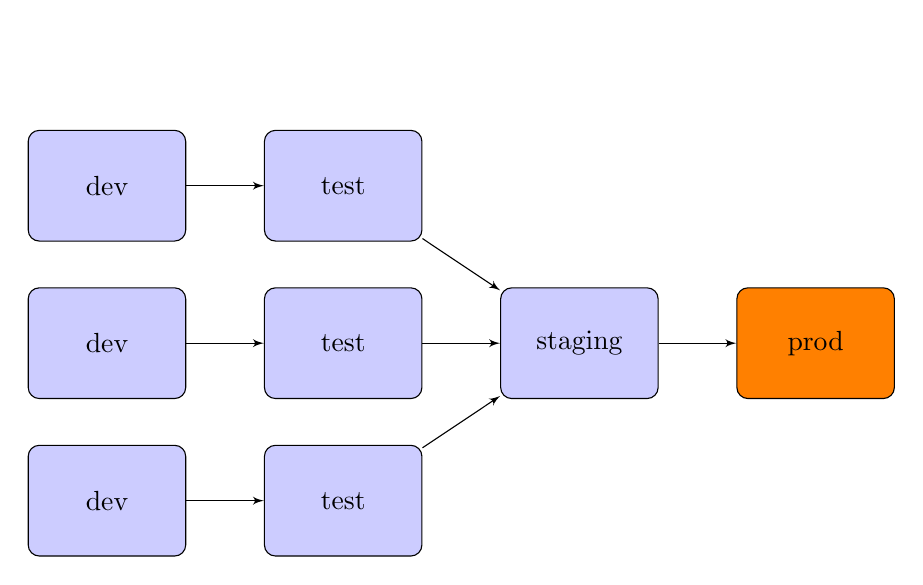
\begin{tikzpicture}[node distance=3cm, minimum size=2cm, auto]
		\node [block, fill=orange] (prod) {prod};
		\node [block, left of=prod] (staging) {staging};
		\node [block, left of=staging] (test) {test};
		\node [block, node distance=2cm, above of=test] (test1) {test};
		\node [block, node distance=2cm, below of=test] (test2) {test};
		\node [block, left of=test] (dev) {dev};
		\node [block, node distance=2cm, above of=dev] (dev1) {dev};
		\node [block, node distance=2cm, below of=dev] (dev2) {dev};
		
		\path [line] (dev) -- node {} (test);
		\path [line] (dev1) -- node {} (test1);
		\path [line] (dev2) -- node {} (test2);
		\path [line] (test) -- node {} (staging);
		\path [line] (test1) -- node {} (staging);
		\path [line] (test2) -- node {} (staging);
		\path [line] (staging) -- node {} (prod);
	\end{tikzpicture}
	
	\ \\
\end{frame}

\begin{frame}[fragile]{Co, gdzie, kiedy, jak?}
	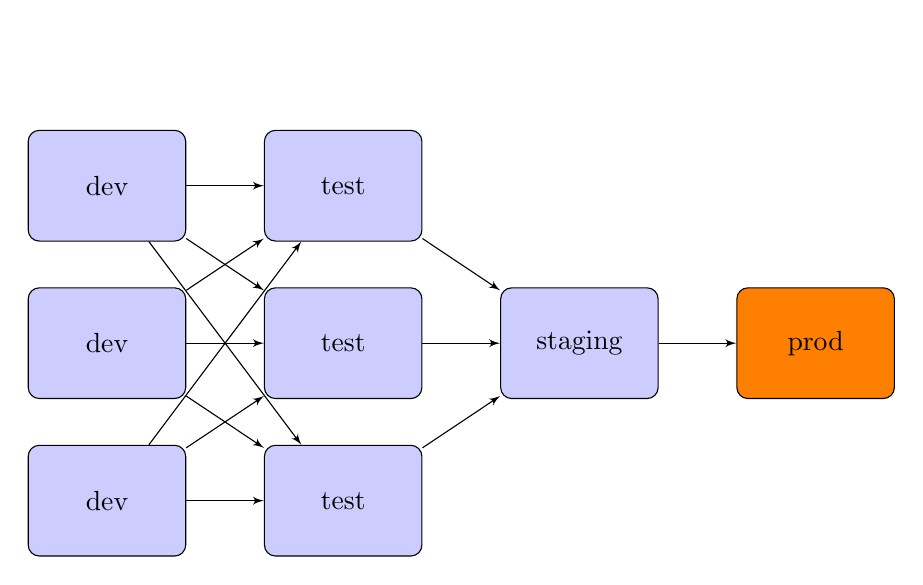
\begin{tikzpicture}[node distance=3cm, minimum size=2cm, auto]
		\node [block, fill=orange] (prod) {prod};
		\node [block, left of=prod] (staging) {staging};
		\node [block, left of=staging] (test) {test};
		\node [block, node distance=2cm, above of=test] (test1) {test};
		\node [block, node distance=2cm, below of=test] (test2) {test};
		\node [block, left of=test] (dev) {dev};
		\node [block, node distance=2cm, above of=dev] (dev1) {dev};
		\node [block, node distance=2cm, below of=dev] (dev2) {dev};
		
		\path [line] (dev) -- node {} (test);
		\path [line] (dev) -- node {} (test1);
		\path [line] (dev) -- node {} (test2);
		\path [line] (dev1) -- node {} (test);
		\path [line] (dev1) -- node {} (test1);
		\path [line] (dev1) -- node {} (test2);
		\path [line] (dev2) -- node {} (test);
		\path [line] (dev2) -- node {} (test1);
		\path [line] (dev2) -- node {} (test2);
		\path [line] (test) -- node {} (staging);
		\path [line] (test1) -- node {} (staging);
		\path [line] (test2) -- node {} (staging);
		\path [line] (staging) -- node {} (prod);
	\end{tikzpicture}
	
	\ \\
\end{frame}

\begin{frame}{Kanon środowisk?}
	Powiązania między środowiskami oczywiście są dowolne, a przede wszystkim powinny zależeć od wymagań klienta. 
	
	Łatwo sobie wyobrazić dodanie dodatkowych węzłów w poprzednio przedstawionych slajdach. Wszystko powinno być jednakże opracowywane z umiarem.
\end{frame}

\section{Środowisko lokalne}

\begin{frame}{Środowisko lokalne}
	\textbf{Środowisko lokalne} to środowisko stacji roboczej przy której pracuje programista.
\end{frame}

\begin{frame}[fragile]{\texttt{ENV=dev}}
	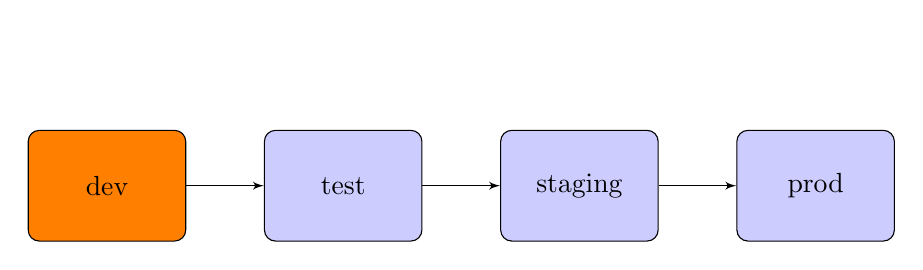
\begin{tikzpicture}[node distance=3cm, minimum size=2cm, auto]
		\node [block] (prod) {prod};
		\node [block, left of=prod] (staging) {staging};
		\node [block, left of=staging] (test) {test};
		\node [block, fill=orange, left of=test] (dev) {dev};
		
		\path [line] (dev) -- node {} (test);
		\path [line] (test) -- node {} (staging);
		\path [line] (staging) -- node {} (prod);
	\end{tikzpicture}
	
	\ \\
\end{frame}

\begin{frame}{Środowisko lokalne}
	Korzystając z wirtualizacji lub konteneryzacji można zbliżyć do tożsamości środowiska deweloperskie i produkcyjne. Jest to sytuacja idealna, ostatnio coraz częściej promowana, jednak niestety wciąż nieczęsto spotykana na rynku pracy.
	
	Prawda jest taka, że dbając o \emph{higienę} programistyczną można spokojnie programować w ulubionych lub dostępnym systemie operacyjnym i środowisku.
	
	Czym powinna być taka \emph{higiena}? Przede wszystkim znajomością różnic między systemami i umiejętnością radzenia sobie z problemami, które mogą z tego wyniknąć. 
\end{frame}

\begin{frame}{Środowisko lokalne}
	Czym się \textbf{może} różnić środowisko lokalne od pozostałych?
	\begin{itemize}
		\item zazwyczaj jest tzw. sandboksem,
		\item posiada bardziej rozbudowane system logów,
		\item ma uruchomione narzędzia deweloperskie: debugbar, profiler, itd.
		\item ma wyłączone lub przekierowane funkcje analizy ruchu,
		\item na nim uruchamiane jest IDE.
	\end{itemize}
\end{frame}

\begin{frame}[fragile]{Przykład}
	\begin{lstlisting}
	
use Phalcon\Mvc\Application;
use Whoops\Provider\Phalcon\WhoopsServiceProvider as Whoops;

error_reporting(E_ALL);

define("APP_PATH", realpath(".."));

require_once APP_PATH . "/vendor/autoload.php";

$config = include APP_PATH . "/app/config.php";
$di = include APP_PATH . "/app/services.php";

$application = new Application($di);

if($config->application->environment == "dev") {
    new Whoops($di);
}

echo $application->handle()->getContent();
	\end{lstlisting}
\end{frame}

\begin{frame}{Przykład}
	\begin{figure}[t]
		\centering
		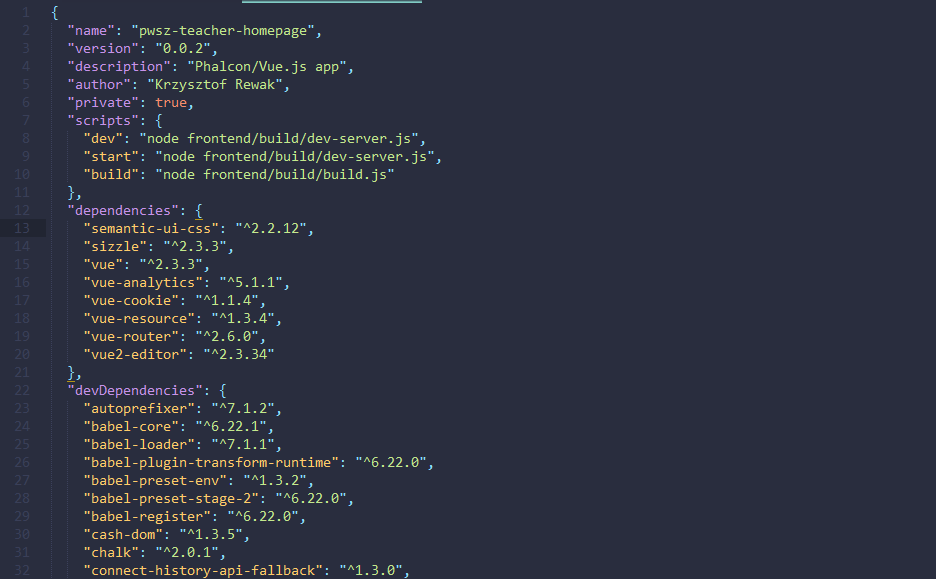
\includegraphics[width=\linewidth]{package.png}
		\caption{Podział na zależności wymagane dla środowiska deweloperskiego oraz innych}
	\end{figure}
\end{frame}

\section{Środowisko testowe}

\begin{frame}{Środowisko testowe}
	\textbf{Środowisko testowe} może funkcjonować zarówno jako drugie środowisko na maszynie deweloperskiej lub jako osobny byt. Jego celem jest uruchomienie wszelkiego rodzaju testów, które sprawdzają czy aplikacja działa w poprawny sposób.
\end{frame}

\begin{frame}[fragile]{\texttt{ENV=test}}
	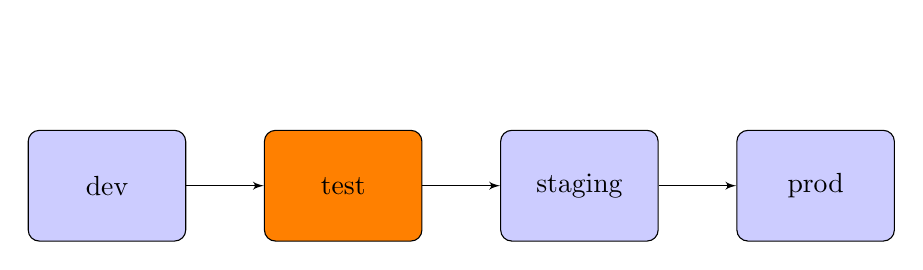
\begin{tikzpicture}[node distance=3cm, minimum size=2cm, auto]
		\node [block] (prod) {prod};
		\node [block, left of=prod] (staging) {staging};
		\node [block, fill=orange, left of=staging] (test) {test};
		\node [block, left of=test] (dev) {dev};
		
		\path [line] (dev) -- node {} (test);
		\path [line] (test) -- node {} (staging);
		\path [line] (staging) -- node {} (prod);
	\end{tikzpicture}
	
	\ \\
\end{frame}

\begin{frame}{Jak to działa od strony repozytorium?}
	Bez względu na wybrany sposób dzielenia gałęzi repozytorium projektu, dobrą praktyką jest utworzenie gałęzi głównej, ale nie będącej gałęzią \texttt{master}, która \emph{zazwyczaj} jest zarezerwowana na ostateczny kod trafiający na serwer produkcjny.
\end{frame}

\begin{frame}{Jak to działa od strony repozytorium?}
	Przykładowo dobrym pomysłem może być utworzenie gałęzi \emph{dev}, do której progamiści będą włączać wszystkie swoje zmiany. Taką gałąź warto przetestować zanim aplikacja zostanie wypuszczona w świat.
\end{frame}

\begin{frame}[fragile]{Ale jakie testy?}
	Obecnie najpopularniejszym i na pewno wartym do poznania sposobem testowania aplikacji są \textbf{testy jednostkowe}. 
	
	Polegają - zgodnie z nazwą - na sprawdzaniu czy pojedyncze elementy aplikacji działają poprawnie. Elementami takimi mogą być metody, obiekty lub nawet grupy obiektow.
\end{frame}

\begin{frame}[fragile]{Testy jednostkowe}
	\begin{lstlisting}
[TestMethod]  
public void Withdraw_ValidAmount_ChangesBalance()  
{  
    // arrange  
    double currentBalance = 10.0;  
    double withdrawal = 1.0;  
    double expected = 9.0;  
    var account = new CheckingAccount("JohnDoe", currentBalance);  
    
    // act  
    account.Withdraw(withdrawal);  
    double actual = account.Balance;  
    
    // assert  
    Assert.AreEqual(expected, actual);  
} 
	\end{lstlisting}
\end{frame}

\begin{frame}{Pliki środowiskowe}
	Niektóre frameworki bazują na plikach \texttt{.env}, w których w wygodny sposób można przetrzymywać istotne dane. Zasada mówi, że każde środowisko powinno mieć swój własny plik środowiskowy.
	
	Ważnym jest zatem, aby nie dodawać ich nigdy do repozytorium, ponieważ zawierają dane, które a) będą niepoprawne dla różnych maszyn i b) niekoniecznie powinny być publiczne ze względów bezpieczeństwa.
\end{frame}

\begin{frame}[fragile]{Pliki środowiskowe}
\begin{columns}
\begin{column}{0.5\textwidth}
\begin{lstlisting}
ENV=dev

APP_KEY=7dbba255-1c7d-46b4-8c5a
APP_URL=http://pwsz.local/

DATABASE_HOST=localhost
DATABASE_USERNAME=root
DATABASE_PASSWORD=alohomora
DATABASE_NAME=pwsz

LOGGER_LEVEL=debug
LOGGER_DRIVER=file
\end{lstlisting}
\end{column}
\begin{column}{0.5\textwidth}
\begin{lstlisting}
ENV=test

APP_KEY=b0f246b4-9f0a-43b0-a922
APP_URL=http://test.pwsz.local/

DATABASE_HOST=localhost
DATABASE_USERNAME=root
DATABASE_PASSWORD=alohomora
DATABASE_NAME=pwsz-test

LOGGER_LEVEL=error
LOGGER_DRIVER=file
\end{lstlisting}
\end{column}
\end{columns}
\end{frame}

\begin{frame}{Co dalej?}
	Dopiero gdy przejdą wszystkie testy automatyczne, najlepiej na środowisku lokalnym i testowym, aplikacja powinna zostać \emph{pchnięta} dalej.
	
	Istnieje kilka sposobów, aby dostarczyć zmiany na serwer:
	\begin{itemize}
		\item najgorszy: FTP lub SCP
		\item najpopularniejszy: git pull
		\item najlepszy: CI
	\end{itemize}
\end{frame}

\section{Środowisko stagingowe}

\begin{frame}{Środowisko stagingowe}
	\textbf{Środowisko stagingowe} to pewnego rodzaju pokaz prapremierowy aplikacji. Na \emph{scenie} uruchamiane są wszystkie procesy podłączone do własnych serwisów i zasobów, a klient ma możliwość sprawdzić czy wszystko działa, wygląda i zachowuje się tak jak powinno.
\end{frame}

\begin{frame}[fragile]{\texttt{ENV=staging}}
	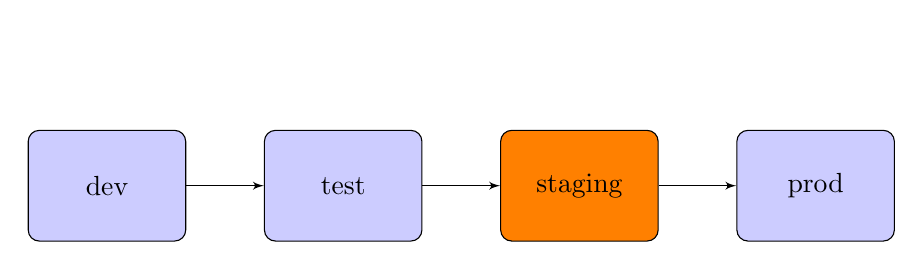
\begin{tikzpicture}[node distance=3cm, minimum size=2cm, auto]
		\node [block] (prod) {prod};
		\node [block, fill=orange, left of=prod] (staging) {staging};
		\node [block, left of=staging] (test) {test};
		\node [block, left of=test] (dev) {dev};
		
		\path [line] (dev) -- node {} (test);
		\path [line] (test) -- node {} (staging);
		\path [line] (staging) -- node {} (prod);
	\end{tikzpicture}
	
	\ \\
\end{frame}

\begin{frame}{Środowisko stagingowe}
	Czasami:
	\begin{itemize}
		\item programista wykonał wszystko zgodnie z dostarczoną specyfikacją projektu,
		\item wszystkim w zespole wydaje się, że wszystko jest okej,
		\item kod ma 100\% pokrycia testami i wszystkie testy przechodzi śpiewająco...
	\end{itemize}
	
	... a i tak biznes odrzuci nową wersję aplikacji.
\end{frame}

\begin{frame}{Środowisko stagingowe}
	Powodów może być mnóstwo:
	
	\begin{itemize}
		\item źle zrozumiany i zaimplementowany proces,
		\item nowe warunki walidacji,
		\item brak integracji z istniejącymi dotąd danymi,
		\item brzydki font, zły kolor przycisku, zbyt duży margines...
	\end{itemize}
\end{frame}

\begin{frame}{Środowisko stagingowe}
	O ileż lepiej przeprowadzić tak zwane testy manualne i mieć stuprocentową pewność, że wszystko jest okej?
	
	Z tego powodu środowiska stagingowe wystawia się na publiczny serwer HTTP, często pod osłoną \texttt{.htaccess} lub innego sposobu uwierzytelniania, często pod domeną \texttt{beta.nazwastrony.pl} lub \texttt{test.nazwastrony.pl}, ale praktycznie zawsze na maszynie identycznej do tej, na której stoi serwer produkcyjny.
\end{frame}

\begin{frame}{Środowisko stagingowe}
	To w tym miejscu administracja aplikacji może poznać nowe funkcjonalności, a upoważniona osoba odebrać zamówione zmiany.
\end{frame}

\begin{frame}{Środowisko stagingowe}
	Oczywiście środowisko stagingowe powinno być wciąż w pewien sposób odseparowane od \emph{prawdziwego świata}. Z tego powodu chociażby:
	\begin{itemize}
		\item bazy danych seeduje się adresami email w domenie własnej firmy lub \texttt{@example.com},
		\item wyłączone lub podpięte pod inny klucz są analityki i śledzenia klientów,
		\item wciąż czasami włączone są powiadomienia serwisowe o błędach,
		\item ustawiony jest wyższy poziom zapisywania logów.
	\end{itemize}
\end{frame}

\begin{frame}{Środowisko stagingowe}
	Jeżeli jednak wszystko gra, aplikacja powinna trafić na serwer produkcyjny już bez problemów.
\end{frame}

\section{Środowisko produkcyjne}

\begin{frame}{Środowisko produkcyjne}
	\textbf{Środowisko produkcyjne} to ostatnia stacja na trasie wdrażania systemu internetowego. Jest to maszyna lub klaster maszyn, które są dostępne dla całego świata. Tutaj nie ma już miejsca na błędy i szybkie hotfiksy.
\end{frame}

\begin{frame}[fragile]{\texttt{ENV=prod}}
	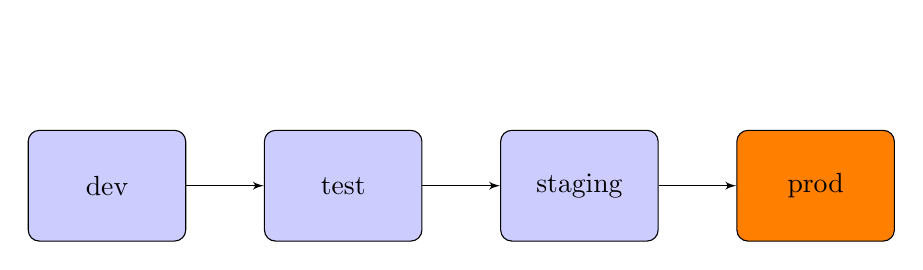
\begin{tikzpicture}[node distance=3cm, minimum size=2cm, auto]
		\node [block, fill=orange] (prod) {prod};
		\node [block, left of=prod] (staging) {staging};
		\node [block, left of=staging] (test) {test};
		\node [block, left of=test] (dev) {dev};
		
		\path [line] (dev) -- node {} (test);
		\path [line] (test) -- node {} (staging);
		\path [line] (staging) -- node {} (prod);
	\end{tikzpicture}
	
	\ \\
\end{frame}

\begin{frame}{Środowisko produkcyjne}
	Proces aktualizacji środowiska produkcyjnego powinien być zawsze przemyślany.
	
	Istnieją sposoby, aby zrobić aktualizację oprogramowania (czasami wraz z testami!) w czasie coraz bardziej dążącym do zera. Jednym z takich rozwiązać jest \emph{blue-green deployment}.
\end{frame}

\begin{frame}{Środowisko produkcyjne}
	Jeżeli jednak z jakiegokolwiek powodu deploy robiony jest ręcznie, należy zrobić to w najodpowiedniejszej chwili:
	\begin{itemize}
		\item w godzinie najmniejszego obłożenia według logów serwera lub analityk wejść,
		\item w uprzednio zapowiedzianym czasie,
		\item w terminie, który pasuje klientowi.
	\end{itemize}
	
	Niestety nie ma jednego gotowego scenariusza, który pasowałby do każdego projektu.
\end{frame}

\section{Podsumowanie}

\begin{frame}{Bibliografia i ciekawe źródła}
  
	\begin{thebibliography}{9}
		
		\bibitem{deployment}
		\url{https://en.wikipedia.org/wiki/Deployment_environment}
	
		\bibitem{unit}
		\url{https://msdn.microsoft.com/en-us/library/hh694602.aspx}
		
		\bibitem{env}
		\url{https://docs.docker.com/compose/env-file/}
		
		\bibitem{bgd}
		\url{https://martinfowler.com/bliki/BlueGreenDeployment.html}
		
	\end{thebibliography}

\end{frame}

\appendix

\begin{frame}[standout]
	Pytania?
\end{frame}

\begin{frame}{}

	Kod prezentacji dostępny jest w repozytorium git pod adresem \texttt{https://bitbucket.org/krewak/pwsz-ppsi} \\ \ \\

	\begin{figure}
		\centering
		\href{https://bitbucket.org/krewak/pwsz-ppsi}{
			
\includegraphics[width=.15\textwidth]{../_template/bitbucket.png}
		}
	\end{figure}
	
	Wszystkie informacje dot. kursu dostępne są pod adresem \texttt{http://pwsz.rewak.pl/kursy/4} \\ \ \\

	\begin{figure}
		\centering
		\href{http://pwsz.rewak.pl/kursy/3}{
			
\includegraphics[width=.15\textwidth]{../_template/rewak.png}
		}
	\end{figure}

\end{frame}

\end{document}
